\documentclass{article}
\usepackage[automake, acronym, nonumberlist, nopostdot]{glossaries}
\usepackage{cite}
\usepackage{hyperref}
\usepackage{listings}
\usepackage{chngcntr}
\usepackage{graphicx}
\usepackage[T1]{fontenc}
\usepackage[utf8]{inputenc}
\usepackage{proof}
\graphicspath{ {./img/} }
\numberwithin{equation}{section}

\lstset
{
	basicstyle=\small\ttfamily,
	frame=bt,
	numbers=left,
	tabsize=2,
	captionpos=b,
	aboveskip=2em,
	belowskip=2em
}

%%%%%%%%%%%%%%%%%%%%%%%%%%%%%%%%%%%%%%%%%%%%%%%%%%%%%%%%%%%%%%%%%%%%%%%%%%%%%%%%%%%%%%%%%%
%%%%%%%%%%%%%%%%%%%%%%%%%%%%%%%%%%%%%%%%%%%%%%%%%%%%%%%%%%%%%%%%%%%%%%%%%%%%%%%%%%%%%%%%%%
%%%%%
%%%%%	Commands
%%%%%
%%%%%%%%%%%%%%%%%%%%%%%%%%%%%%%%%%%%%%%%%%%%%%%%%%%%%%%%%%%%%%%%%%%%%%%%%%%%%%%%%%%%%%%%%%
%%%%%%%%%%%%%%%%%%%%%%%%%%%%%%%%%%%%%%%%%%%%%%%%%%%%%%%%%%%%%%%%%%%%%%%%%%%%%%%%%%%%%%%%%%
		
\renewcommand{\lstlistingname}{Code listing}
\renewcommand{\lstlistlistingname}{List of code listings}

\newcommand{\mstate}[2]{
	\langle#1, #2\rangle
}

\newcommand{\ipointsto}[2] {
	#1 \nearrow \texttt{#2}
}

\newcommand{\sval}[2] {
	#1_\texttt{#2}
}

%%%%%%%%%%%%%%%%%%%%%%%%%%%%%%%%%%%%%%%%%%%%%%%%%%%%%%%%%%%%%%%%%%%%%%%%%%%%%%%%%%%%%%%%%%
%%%%%%%%%%%%%%%%%%%%%%%%%%%%%%%%%%%%%%%%%%%%%%%%%%%%%%%%%%%%%%%%%%%%%%%%%%%%%%%%%%%%%%%%%%
%%%%%
%%%%%	Create acronyms
%%%%%
%%%%%%%%%%%%%%%%%%%%%%%%%%%%%%%%%%%%%%%%%%%%%%%%%%%%%%%%%%%%%%%%%%%%%%%%%%%%%%%%%%%%%%%%%%
%%%%%%%%%%%%%%%%%%%%%%%%%%%%%%%%%%%%%%%%%%%%%%%%%%%%%%%%%%%%%%%%%%%%%%%%%%%%%%%%%%%%%%%%%%

\newacronym{cil}{CIL}{Common Intermediate Language}
\newacronym{msil}{MSIL}{Microsoft Intermediate Language}
\newacronym{il}{IL}{Intermediate Language}
\newacronym{cli}{CLI}{Common Language Infrastructure}
\newacronym{iso}{ISO}{International Organization for Standardization}
\newacronym{cts}{CTS}{Common Type System}
\newacronym{cls}{CLS}{Common Language Specification}
\newacronym{ves}{VES}{Virtual Execution System}
\newacronym{ast}{AST}{Abstract syntax tree}
\makeglossaries

%%%%%%%%%%%%%%%%%%%%%%%%%%%%%%%%%%%%%%%%%%%%%%%%%%%%%%%%%%%%%%%%%%%%%%%%%%%%%%%%%%%%%%%%%%
%%%%%%%%%%%%%%%%%%%%%%%%%%%%%%%%%%%%%%%%%%%%%%%%%%%%%%%%%%%%%%%%%%%%%%%%%%%%%%%%%%%%%%%%%%
%%%%%
%%%%%	Begin document
%%%%%
%%%%%%%%%%%%%%%%%%%%%%%%%%%%%%%%%%%%%%%%%%%%%%%%%%%%%%%%%%%%%%%%%%%%%%%%%%%%%%%%%%%%%%%%%%
%%%%%%%%%%%%%%%%%%%%%%%%%%%%%%%%%%%%%%%%%%%%%%%%%%%%%%%%%%%%%%%%%%%%%%%%%%%%%%%%%%%%%%%%%%

\begin{document}
\counterwithin{lstlisting}{section}

%%%%%%%%%%%%%%%%%%%%%%%%%%%%%%%%%%%%%%%%%%%%%%%%%%%%%%%%%%%%%%%%%%%%%%%%%%%%%%%%%%%%%%%%%%
%%%%%%%%%%%%%%%%%%%%%%%%%%%%%%%%%%%%%%%%%%%%%%%%%%%%%%%%%%%%%%%%%%%%%%%%%%%%%%%%%%%%%%%%%%
%%%%%
%%%%%	Contents
%%%%%
%%%%%%%%%%%%%%%%%%%%%%%%%%%%%%%%%%%%%%%%%%%%%%%%%%%%%%%%%%%%%%%%%%%%%%%%%%%%%%%%%%%%%%%%%%
%%%%%%%%%%%%%%%%%%%%%%%%%%%%%%%%%%%%%%%%%%%%%%%%%%%%%%%%%%%%%%%%%%%%%%%%%%%%%%%%%%%%%%%%%%

\tableofcontents
\clearpage

%%%%%%%%%%%%%%%%%%%%%%%%%%%%%%%%%%%%%%%%%%%%%%%%%%%%%%%%%%%%%%%%%%%%%%%%%%%%%%%%%%%%%%%%%%
%%%%%%%%%%%%%%%%%%%%%%%%%%%%%%%%%%%%%%%%%%%%%%%%%%%%%%%%%%%%%%%%%%%%%%%%%%%%%%%%%%%%%%%%%%
%%%%%
%%%%%	Acronyms
%%%%%
%%%%%%%%%%%%%%%%%%%%%%%%%%%%%%%%%%%%%%%%%%%%%%%%%%%%%%%%%%%%%%%%%%%%%%%%%%%%%%%%%%%%%%%%%%
%%%%%%%%%%%%%%%%%%%%%%%%%%%%%%%%%%%%%%%%%%%%%%%%%%%%%%%%%%%%%%%%%%%%%%%%%%%%%%%%%%%%%%%%%%

\printglossary[type=\acronymtype]
\clearpage

%%%%%%%%%%%%%%%%%%%%%%%%%%%%%%%%%%%%%%%%%%%%%%%%%%%%%%%%%%%%%%%%%%%%%%%%%%%%%%%%%%%%%%%%%%
%%%%%%%%%%%%%%%%%%%%%%%%%%%%%%%%%%%%%%%%%%%%%%%%%%%%%%%%%%%%%%%%%%%%%%%%%%%%%%%%%%%%%%%%%%
%%%%%
%%%%%	Figures
%%%%%
%%%%%%%%%%%%%%%%%%%%%%%%%%%%%%%%%%%%%%%%%%%%%%%%%%%%%%%%%%%%%%%%%%%%%%%%%%%%%%%%%%%%%%%%%%
%%%%%%%%%%%%%%%%%%%%%%%%%%%%%%%%%%%%%%%%%%%%%%%%%%%%%%%%%%%%%%%%%%%%%%%%%%%%%%%%%%%%%%%%%%

\listoffigures
\clearpage

%%%%%%%%%%%%%%%%%%%%%%%%%%%%%%%%%%%%%%%%%%%%%%%%%%%%%%%%%%%%%%%%%%%%%%%%%%%%%%%%%%%%%%%%%%
%%%%%%%%%%%%%%%%%%%%%%%%%%%%%%%%%%%%%%%%%%%%%%%%%%%%%%%%%%%%%%%%%%%%%%%%%%%%%%%%%%%%%%%%%%
%%%%%
%%%%%	Code listings
%%%%%
%%%%%%%%%%%%%%%%%%%%%%%%%%%%%%%%%%%%%%%%%%%%%%%%%%%%%%%%%%%%%%%%%%%%%%%%%%%%%%%%%%%%%%%%%%
%%%%%%%%%%%%%%%%%%%%%%%%%%%%%%%%%%%%%%%%%%%%%%%%%%%%%%%%%%%%%%%%%%%%%%%%%%%%%%%%%%%%%%%%%%

\lstlistoflistings
\clearpage

%%%%%%%%%%%%%%%%%%%%%%%%%%%%%%%%%%%%%%%%%%%%%%%%%%%%%%%%%%%%%%%%%%%%%%%%%%%%%%%%%%%%%%%%%%
%%%%%%%%%%%%%%%%%%%%%%%%%%%%%%%%%%%%%%%%%%%%%%%%%%%%%%%%%%%%%%%%%%%%%%%%%%%%%%%%%%%%%%%%%%
%%%%%
%%%%%	Introduction
%%%%%
%%%%%%%%%%%%%%%%%%%%%%%%%%%%%%%%%%%%%%%%%%%%%%%%%%%%%%%%%%%%%%%%%%%%%%%%%%%%%%%%%%%%%%%%%%
%%%%%%%%%%%%%%%%%%%%%%%%%%%%%%%%%%%%%%%%%%%%%%%%%%%%%%%%%%%%%%%%%%%%%%%%%%%%%%%%%%%%%%%%%%

\section{Introduction}

\subsection{The \acrlong{cli}}

\textit{The \acrfull{cli}} is a specification developed by \textit{Microsoft} and standardized by \textit{\acrshort{iso}} and \textit{ECMA International} \cite{isoStandard, ecmaStandard}. It describes executable code and an environment that allows numerous programming languages to be executed on various platforms.

The following four main aspects are covered by the \acrlong{cli} \cite{ecmaStandard}:
\begin{itemize}
	\item{
		\textbf{\textit{The \acrfull{cts}}} - a type system supporting types and operations found in many programming languages;
	}
	\item{
		\textbf{Metadata} - used for describing and referencing types defined by the \acrshort{cts};
	}
	\item{
		\textbf{\textit{The \acrfull{cls}}} - an agreement between language designers and framework designers specifying a subset of the \acrshort{cts} and a set of usage conventions;
	}
	\item{
		\textbf{\textit{The \acrfull{ves}}} - responsible for loading and executing programs written for the \acrshort{cli}.
	}
\end{itemize}

There are multiple implementations of the \acrshort{cli}, for instance: \textit{.NET Framework}, \textit{Shared Source Common Language Infrastructure Implementation}, \textit{.NET Core} and \textit{Mono}.

\subsection{The \acrlong{cil}}

\textit{The \acrfull{cil}} is also known as \textit{the \acrfull{msil}} or simply \textit{the \acrfull{il}} \cite{procsharp7}. It is an object-oriented programming language that is a part of the \acrshort{cli}. Each language compatible with the \acrshort{cli} is compiled into the \acrshort{cil}. Moreover, the \acrshort{cil} is the actual language executed by the \acrshort{ves}. The language is a reasonable compromise between user-friendly, high-level programming languages and low-level assemblers. Although the \acrshort{cil} is human-readable, it is still a stack-based language and writing programs manually is therefore quite difficult.

Technically, the \acrshort{cil} is just a set of over 200 instructions and it does not define a syntax for describing \textit{the \acrshort{cli} metadata}. There is another syntax called \textit{ILAsm} - an assembly language for the \acrshort{cil} \cite{ecmaStandard}. However, many sources refer to the \acrshort{cil} and ILAsm interchangeably. Thus, \textit{the \acrshort{cil}} means hereinafter the whole ILAsm syntax and \textit{the \acrshort{cil} instruction set} refers to the correct meaning of the \acrlong{cil}.

\begin{lstlisting}[
	caption={\textit{Hello world} program.},
	label={lst:hello_world}
]
.assembly extern mscorlib {}

.assembly HelloWorld {}

.method static public void main() cil managed
{
	.entrypoint
	.maxstack 1
	ldstr "Hello world!"
	call void [mscorlib]System.Console::WriteLine(string)
	ret
}
\end{lstlisting}

The difference between ILAsm and the \acrshort{cil} can be easily understood by analysing the \textit{Hello world} program shown in code listing \ref{lst:hello_world}. Lines 1-8 and 12 of the example contain the \acrshort{cli} metadata described in ILasm syntax whereas lines 9-11 contain actual \acrshort{cil} instructions. The detailed meaning of each line can be explained as follows:
\begin{itemize}
	\item{Line 1 informs that an external assembly (\texttt{mscorlib}) should be loaded.}
	\item{Line 3 defines the assembly that should be created as the result of the compiler.}
	\item{Line 5 declares a static public method (\texttt{main}). It also defines that the method contains \acrshort{cil} code.}
	\item{Line 6 begins the body of the \texttt{main} method.}
	\item{Line 7 informs that the method should be used as the entry point of the program - it should be called by the compiler as the very first method.}
	\item{Line 8 specifies the maximal size of the evaluation stack associated with the method.}
	\item{Line 9 contains a \texttt{ldstr} instruction. It tells the compiler to put the \textit{Hello world!} string onto the evaluation stack.}
	\item{Line 10 contains a \texttt{call} instruction. It tells the compiler to call the \texttt{WriteLine} method from the \texttt{System.Console} class defined in the \texttt{mscorlib} assembly.}
	\item{Line 11 contains a \texttt{ret} instruction. It tells the compiler to return the result of the method and to transfer the control to the next method on the call stack.}
	\item{Line 12 ends the body of the \texttt{main} method.}
\end{itemize}

\subsection{{\#\#\# TO DO: ZALOZENIA, CEL PRACY I ZAKONCZENIE WSTEPU \#\#\#}}

\clearpage

%%%%%%%%%%%%%%%%%%%%%%%%%%%%%%%%%%%%%%%%%%%%%%%%%%%%%%%%%%%%%%%%%%%%%%%%%%%%%%%%%%%%%%%%%%
%%%%%%%%%%%%%%%%%%%%%%%%%%%%%%%%%%%%%%%%%%%%%%%%%%%%%%%%%%%%%%%%%%%%%%%%%%%%%%%%%%%%%%%%%%
%%%%%
%%%%%	The CIL instruction set
%%%%%
%%%%%%%%%%%%%%%%%%%%%%%%%%%%%%%%%%%%%%%%%%%%%%%%%%%%%%%%%%%%%%%%%%%%%%%%%%%%%%%%%%%%%%%%%%
%%%%%%%%%%%%%%%%%%%%%%%%%%%%%%%%%%%%%%%%%%%%%%%%%%%%%%%%%%%%%%%%%%%%%%%%%%%%%%%%%%%%%%%%%%

\section{The \acrshort{cil} instruction set}

In order to understand how the \acrshort{cil} instructions work, this section explains the concept of the global state and provides code examples introducing several \acrshort{cil} instructions. As the whole set contains more than 200 instructions, further information on each of them can be found in \cite{ecmaStandard} and \cite{isoStandard}.

\subsection{The global state}
\label{sec:global_state}

The \acrshort{cli} can manage multiple threads of control at the same time. A single thread of control can be thought as a call stack consisting of multiple method states. Although all the threads of control are rather independent, they still can access multiple managed heaps allocated in the shared memory space \cite{ecmaStandard}. This concept is presented in figure \ref{fig:global_state}.

\begin{figure}
	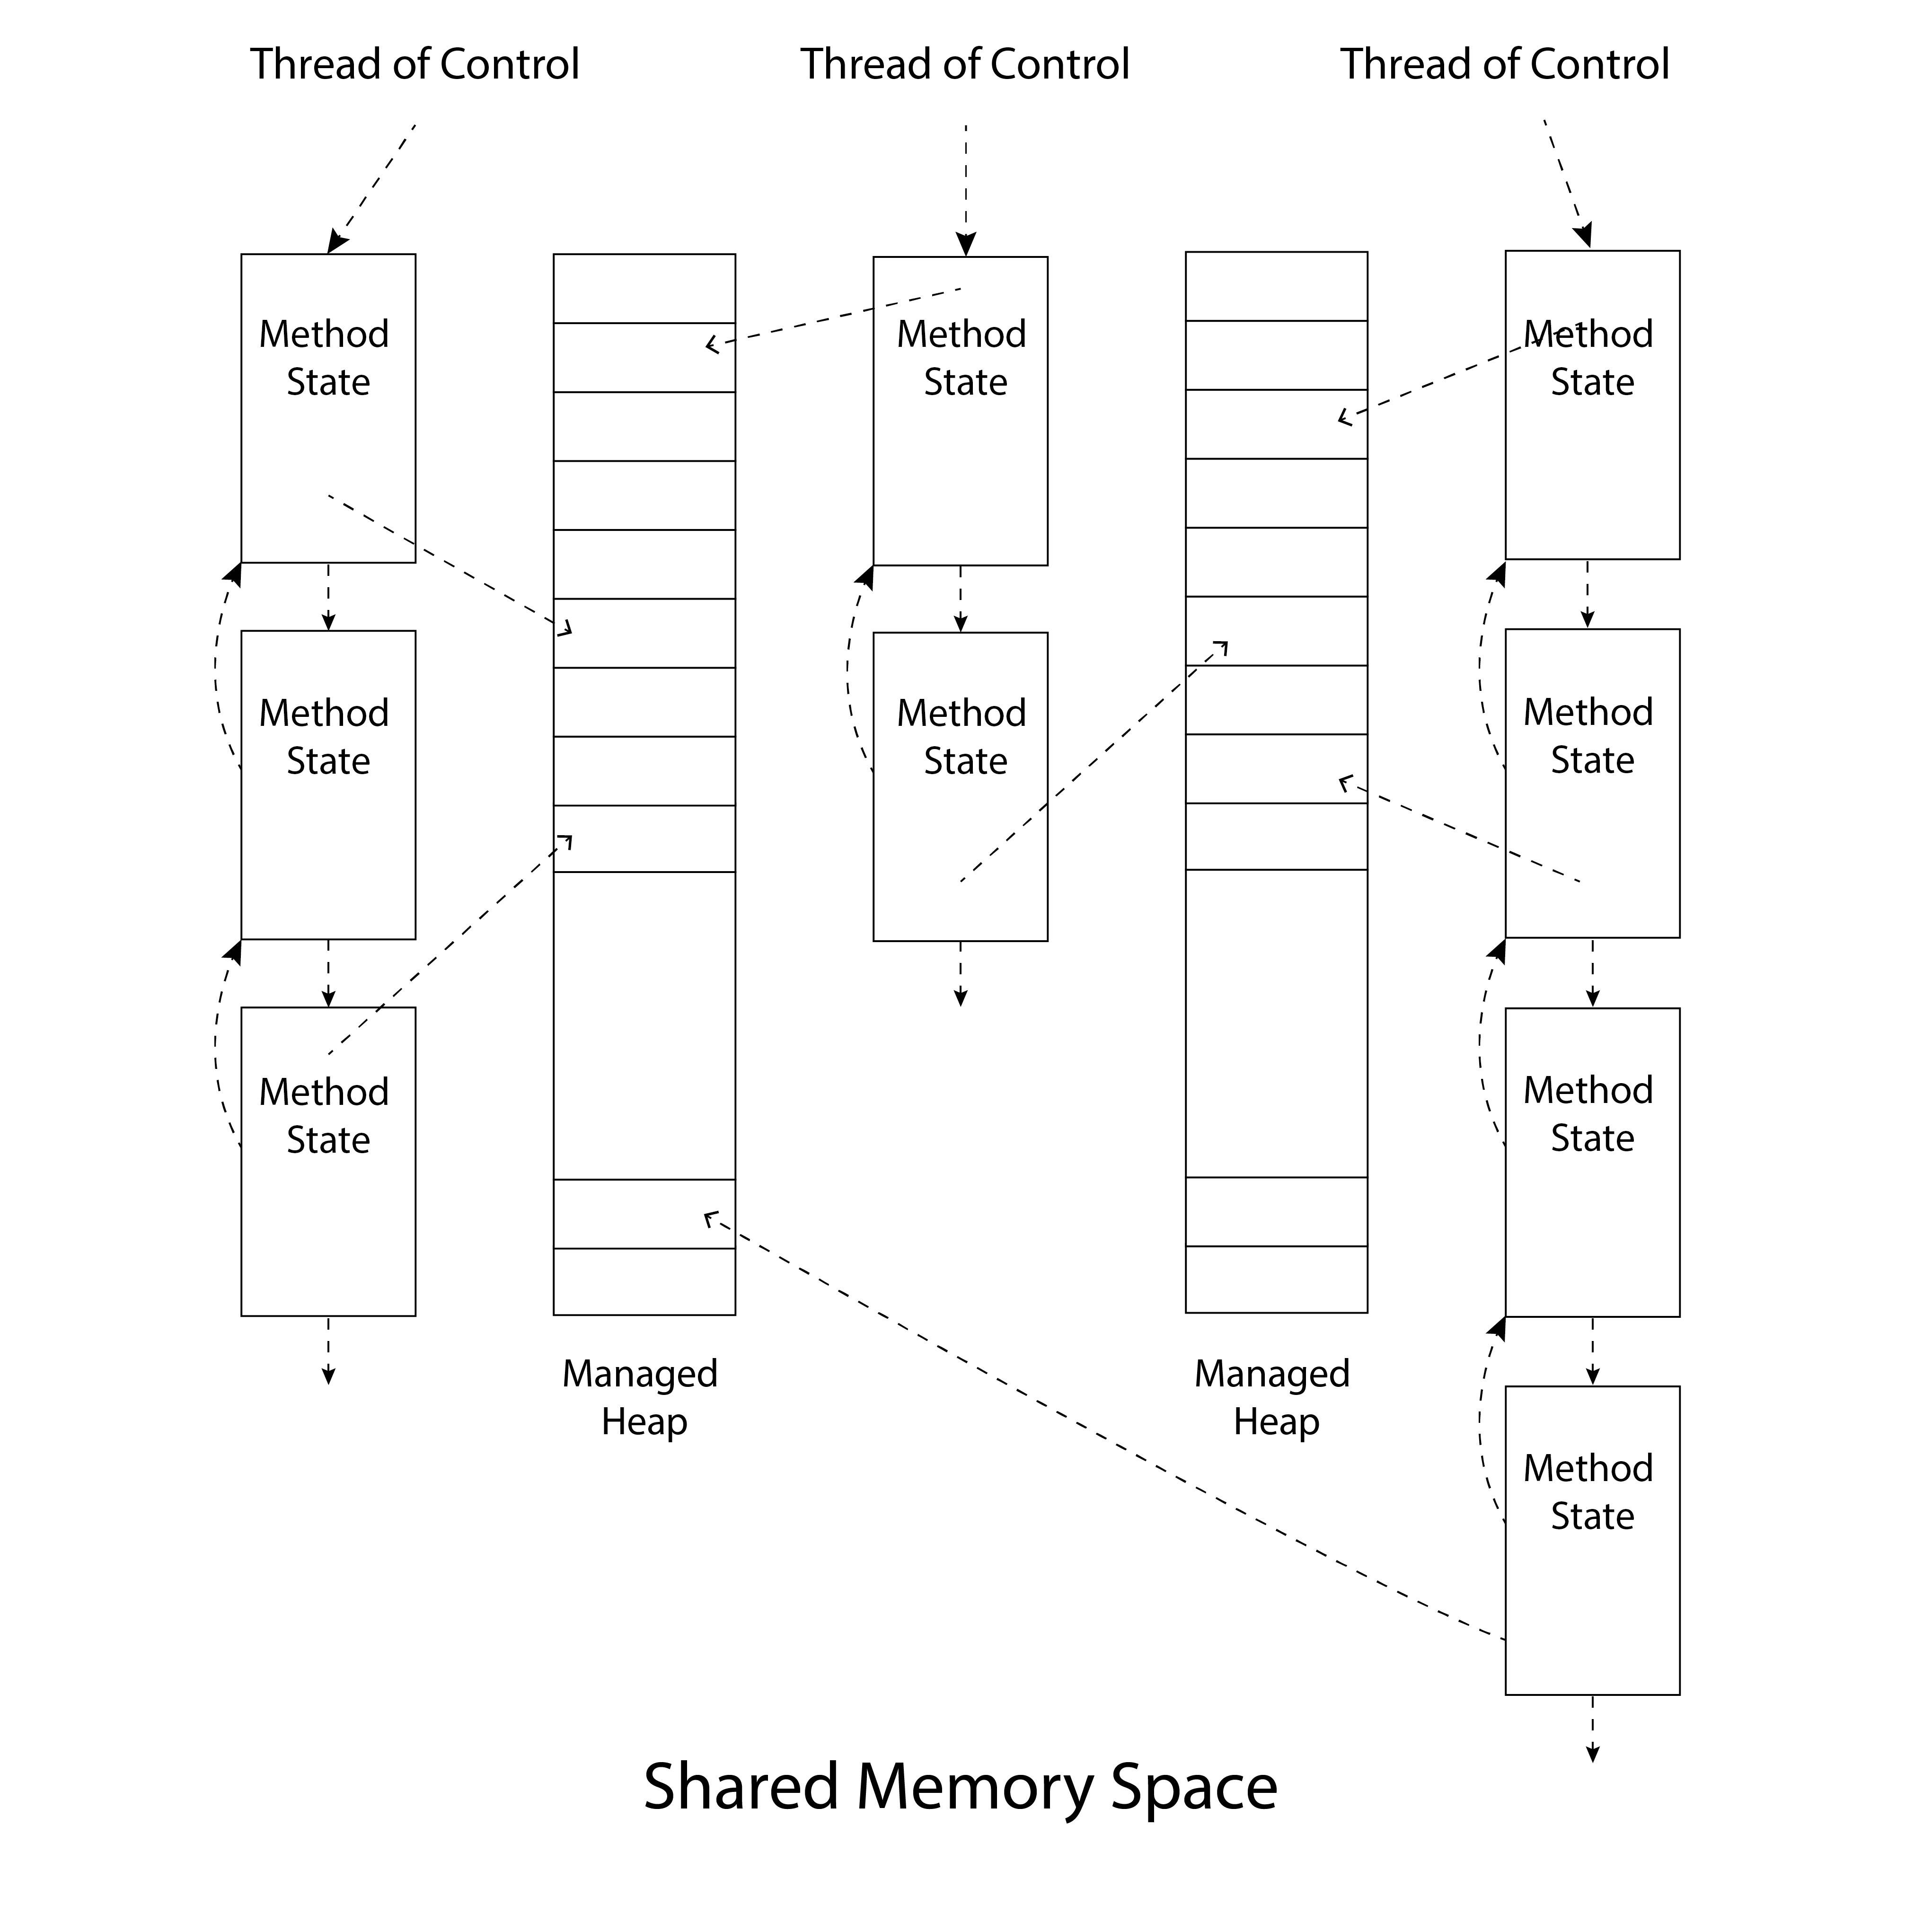
\includegraphics[width=1\textwidth]{global_state.png}
    \centering
    \caption{The global state concept.}
    \label{fig:global_state}
\end{figure}

A single method state includes several items required for the \acrshort{ves} to execute the method \cite{ecmaStandard}, inter alia:
\begin{itemize}
	\item{an instruction pointer - it determines the next instruction that should be executed within the method;}
	\item{an evaluation stack - it stores evaluation values;}
	\item{a method information handle - it contains read-only method information;}
	\item{a local variable array;}
	\item{an argument array.}
\end{itemize}

Generally, a single instruction can be understood as a description of how to manipulate the corresponding method state - there are only a few exceptions to this rule. Some instructions only require access to the evaluation stack while some do need to change other parts of the global state. To better understand these differences, the examples below present a couple of instructions and describe what effect they have on the global state.

\subsection{The evaluation stack}

As described above, a method state contains an evaluation stack. While a rich set of data types can be represented in memory, only a very limited subset of those types are supported by the \acrshort{cli} on an evaluation stack. This subset consists of the following data types \cite{ecmaStandard}:
\begin{itemize}
	\item{\texttt{int32},}
	\item{\texttt{int64},}
	\item{\texttt{native int},}
	\item{\texttt{F} (a floating-point number),}
	\item{\texttt{O} (an object reference),}
	\item{\texttt{\&} (a managed pointer),}
	\item{\texttt{native unsigned int} (also an unmanaged pointer),}
	\item{a user-defined value type.}
\end{itemize}

\subsection{Stack transformations}
\label{sec:stackTransformations}

A stack transformation can be thought as a sequence of pop and / or push operations performed on an evaluation stack. The majority of the \acrshort{cil} instructions uses such a sequence to get some values from the corresponding stack or to push some values onto it. In order to describe and visualise the effect of an instruction, the following syntax is used:
\begin{itemize}
	\item{$S$ denotes an evaluation stack;}
	\item{$S \rightarrow S \cdot v_1 \cdot v_2 \cdot ... \cdot v_n$ denotes a stack transformation which is equivalent to pushing the values $v_1, v_2, ..., v_n$ onto the stack $S$;}
	\item{$S \cdot u_1 \cdot u_2 \cdot ... \cdot u_n \rightarrow S$ denotes a stack transformation which is equivalent to popping the values $u_1, u_2, ..., u_n$ from the stack $S$;}
	\item{$S \cdot u_1 \cdot u_2 \cdot ... \cdot u_n \rightarrow S \cdot v_1 \cdot v_2 \cdot ... \cdot v_m$ denotes a stack transformation which is equivalent to popping values $u_1, u_2, ..., u_n$ from the stack $S$ and then pushing the values $v_1, v_2, ..., v_m$ onto it.}
\end{itemize}

\subsection{Stack values}

To illustrate the difference between various stack values, the following syntax represents the value $v$ of the stack type \texttt{type}:
$$
	\sval{v}{type}
$$.
For instance:
\begin{itemize}
	\item{$\sval{0}{int32}$ represents $0$ of type \texttt{int32}}.
\end{itemize}

\subsection{The examples}
\label{sec:instruction_examples}

\subsubsection{\texttt{ldc.i4.0}}
\label{sec:desc_ldci40}

The \texttt{ldc.i4.0} instruction pushes $0$ onto the evaluation stack as \texttt{int32}. The corresponding stack transformation can be presented as follows \cite{ecmaStandard}:
$$
	S \rightarrow S \cdot 0_\texttt{int32}
$$

The program shown in code listing \ref{lst:ldci40} uses the instruction to push $0$ onto the stack and then writes out the top stack value ($0$) using the \texttt{call} instruction.

\begin{lstlisting}[
	caption={Usage of \texttt{ldc.i4.0} instruction.},
	label={lst:ldci40}
]
.assembly extern mscorlib {}

.assembly HelloWorld {}

.method static public void main() cil managed
{
	.entrypoint
	.maxstack 1
	ldc.i4.0
	call void [mscorlib]System.Console::WriteLine(int32)
	ret
}
\end{lstlisting}

The \acrshort{cil} provides a number of similar instructions to push other constant values onto the stack: \texttt{ldc.i4.1}, \texttt{ldc.i4.2}, \texttt{ldc.i4.3}, \texttt{ldc.i4.4}, \texttt{ldc.i4.5}, \texttt{ldc.i4.6}, \texttt{ldc.i4.7}, \texttt{ldc.i4.8} and \texttt{ldc.i4.m1} (or \texttt{ldc.i4.M1}) which pushes $-1$ onto the stack.

\subsubsection{{\#\#\# TO DO: PRZYKLADY UZYCIA INNYCH INSTRUKCJI \#\#\#}}

\clearpage

%%%%%%%%%%%%%%%%%%%%%%%%%%%%%%%%%%%%%%%%%%%%%%%%%%%%%%%%%%%%%%%%%%%%%%%%%%%%%%%%%%%%%%%%%%
%%%%%%%%%%%%%%%%%%%%%%%%%%%%%%%%%%%%%%%%%%%%%%%%%%%%%%%%%%%%%%%%%%%%%%%%%%%%%%%%%%%%%%%%%%
%%%%%
%%%%%	The semantics
%%%%%
%%%%%%%%%%%%%%%%%%%%%%%%%%%%%%%%%%%%%%%%%%%%%%%%%%%%%%%%%%%%%%%%%%%%%%%%%%%%%%%%%%%%%%%%%%
%%%%%%%%%%%%%%%%%%%%%%%%%%%%%%%%%%%%%%%%%%%%%%%%%%%%%%%%%%%%%%%%%%%%%%%%%%%%%%%%%%%%%%%%%%

\section{The semantics}

As described in \ref{sec:global_state}, an instruction can be thought as a description of how to manipulate the current global state. Examples of such informal descriptions can be found in \ref{sec:instruction_examples}. \cite{ecmaStandard} presents further examples but it does not provide any formal way to describe the \acrshort{cil} instructions and their semantics. Thus, one of the goals of the thesis is to introduce a formal, mathematical model to represent the semantics of the \acrshort{cil}.

The semantics presented below is patterned upon the example of the \acrshort{cil} semantics presented in \cite{zychlaThesis}. However, this thesis attempts to simplify it and to represent the semantics on a higher level of abstraction.

\subsection{The global state}

The global state described in \ref{sec:global_state} can be represented as an ordered pair
\begin{equation}
	\sigma = \langle\tau, \eta\rangle
\end{equation}
where $\sigma$ is a global state, $\tau$ is a set of states of the corresponding threads of control and $\eta$ is a set of states of the managed heaps.

The following formula could be potentially used to describe the semantics \cite{wierzbicki}:
\begin{equation}
\label{eq:wierzbickiFormula}
	\langle I, \sigma_1\rangle \rightarrow \sigma_2.
\end{equation}
It can be understood as follows: if the program is in the state $\sigma_1$ and it executes the instruction $I$, the result state is $\sigma_2$. However, formula \ref{eq:wierzbickiFormula} treats the state and the current instruction as separate beings while the global state of the \acrshort{cil} contains the instruction pointer hence the formula can be simplified:
\begin{equation}
\label{eq:wierzbickiFormula2}
	\sigma_1 \rightarrow \sigma_2.
\end{equation}.

\subsection{The execution state}

Since the global state and its mathematical representation can be very complex, this section is to provide a simpler concept called hereinafter \textit{the execution state}. As a single instruction can only change a state of a single thread of control, there is no need to include the whole global state in the semantics. The execution state is then a part of the global state that could be potentially changed by an instruction and can be represented as an ordered pair:
\begin{equation}
\label{eq:executionState}
	\langle\gamma, \eta\rangle
\end{equation}
where $\gamma$ is the corresponding thread of control (its state) and $\eta$ is a set of states of the managed heaps.

The semantics can be now presented as formulas of the following shape:
\begin{equation}
\label{eq:simpleSemantics}
	\langle\gamma_1, \eta_1\rangle \rightarrow \langle\gamma_2, \eta_2\rangle.
\end{equation}
The formula has an analogous meaning to formula \ref{eq:wierzbickiFormula2} however it operates on the execution state while the rest of the global state remains unchanged. For transparency, the angle brackets can be now omitted.

\subsection{The method state}

As mentioned before, the state of a single thread of control can be understood as a call stack of method states. Thus a similar syntax to the one introduced in section \ref{sec:stackTransformations} is used to illustrate the changes made on a call stack. A single method state can be then described using a tuple
\begin{equation}
\label{eq:methodState}
	\langle I, S \rangle
\end{equation}
where:
\begin{itemize}
	\item{$I$ is the instruction pointer},
	\item{$S$ is the evaluation stack}.
\end{itemize}

\#\#\# TO DO: ROZSZERZYĆ OPIS METHOD STATE'U O POZOSTAŁE ELEMENTY \#\#\#

\subsection{The final syntax}

Taken all together, the semantics of the \acrshort{cil} can be represented as a set of formulas of the following shape:
\begin{equation}
\label{eq:finalSyntax}
	\gamma_1 \cdot \mu_{1,1} \cdot ... \cdot \mu_{1,n}, \eta_1 \rightarrow \gamma_2 \cdot \mu_{2,1} \cdot ... \cdot \mu_{2,m}, \eta_2
\end{equation}
where
\begin{itemize}
	\item{$\gamma_1, \gamma_2$ are call stacks,}
	\item{$\mu_{1,1}, ..., \mu_{1,n}, \mu_{2, 1}, ..., \mu_{2, m}$ are method states,}
	\item{$\eta_1, \eta_2$ are sets of managed heaps.}
\end{itemize}

For instance, the following describes a transformation which pushes 0 of type \texttt{int32} onto the evaluation stack of the top method state:
$$
	\gamma \cdot \mstate{I}{S}, \eta \rightarrow \gamma \cdot \mstate{I}{S \cdot 0_\texttt{int32}}, \eta.
$$

\subsection{Instruction pointers}

To show what actually instruction is pointed by the instruction pointer $I$, the following formula is used:
\begin{equation}
	\ipointsto{I}{instruction}.
\end{equation}
No special mathematical syntax is used to describe various instruction types. For example, the following formula means that the instruction pointer $I$ points to a \texttt{ldc.i4.0} instruction:
$$
	\ipointsto{I}{ldc.i4.0}.
$$

Additionally, according to the syntax presented in \cite{zychlaThesis}, $I_n$ denotes hereinafter a pointer to the $n$-th instruction of a method.

\subsection{The examples}

This section follows the informal descriptions contained in \ref{sec:instruction_examples} and uses the conventions described above in order to specify the semantics of several \acrshort{cil} instructions which can be found in formulas \ref{eq:semantics_first}-\ref{eq:semantics_last}.

\begin{equation}
\label{eq:semantics_first}
	\infer{
		\gamma \cdot \mstate{I_n}{S}, \eta
			\rightarrow
		\gamma \cdot \mstate{I_{n+1}}{S \cdot \sval{0}{int32}}, \eta
	}
	{\ipointsto{I_n}{ldc.i4.0}}
\end{equation}

\begin{equation}
\label{eq:semantics_last}
	\infer{
		\gamma \cdot \mstate{I_n}{S}, \eta
			\rightarrow
		\gamma \cdot \mstate{I_{n+1}}{S \cdot \sval{1}{int32}}, \eta
	}
	{\ipointsto{I_n}{ldc.i4.1}}
\end{equation}

\#\#\# TO DO: UZUPELNIC SEMANTYKA KOLEJNYCH INSTRUKCJI ZGODNIE Z SEKCJA 2.5 \#\#\#

\clearpage

%%%%%%%%%%%%%%%%%%%%%%%%%%%%%%%%%%%%%%%%%%%%%%%%%%%%%%%%%%%%%%%%%%%%%%%%%%%%%%%%%%%%%%%%%%
%%%%%%%%%%%%%%%%%%%%%%%%%%%%%%%%%%%%%%%%%%%%%%%%%%%%%%%%%%%%%%%%%%%%%%%%%%%%%%%%%%%%%%%%%%
%%%%%
%%%%%	The interpreter
%%%%%
%%%%%%%%%%%%%%%%%%%%%%%%%%%%%%%%%%%%%%%%%%%%%%%%%%%%%%%%%%%%%%%%%%%%%%%%%%%%%%%%%%%%%%%%%%
%%%%%%%%%%%%%%%%%%%%%%%%%%%%%%%%%%%%%%%%%%%%%%%%%%%%%%%%%%%%%%%%%%%%%%%%%%%%%%%%%%%%%%%%%%

\section{The interpreter}

The main part of this thesis is the interpreter which reads a \acrshort{cil} source code and is able to execute it.

\#\#\# TO DO: KILKA ZDAN / AKAPITOW O TEORII INTERPRETACJI NA PODSTAWIE ZRODEL \#\#\#

\subsection{The lexer and the parser}

\#\#\# TO DO: KILKA ZDAN O GRAMATYCE, TOKENIZACJI, I PARSOWANIU KODU DO AST \#\#\#

\subsection{Technical background}

In order to focus on the semantics of the \acrshort{cil} and not on data types, the interpreter has been written in \texttt{C\#} which is itself compiled into the \acrshort{cil} so it uses the same type system and the same external assemblies. 

The interpreter is a console application based on the \texttt{.NET Framework 4.7.2} so it can be executed in \texttt{Windows} operating system with the appropriate framework installed. The program can be run with the following command line argument:
\begin{itemize}
	\item{\texttt{--fileName} \texttt{\textit{fileName}} - a path to a text file containing the source code to be interpreted.}
\end{itemize}

The standard input, standard output and standard error streams are redirected to the console in order to allow the interpreted program to interact with the user. For instance, the program shown in code listing \ref{lst:hello_world} calls the \texttt{Console.WriteLine} method to write out the \textit{Hello world!} string to the standard output. The interpreter redirects the output therefore the string appears in the console. However, when an interpreter exception is caught, it is also written to the standard error stream.

\subsection{Detection of non-supported features}

Before interpreting the provided source code, the application checks if the code is supported by the interpreter. Once a non-supported feature is detected, one of the following exceptions is thrown and written out to the console:
\begin{itemize}
	\item{\texttt{InstructionNotSupportedException},}
	\item{\texttt{FeatureNotSupportedException}.}
\end{itemize}

\subsection{The actual interpreter}

In order to implement the interpreter, a couple of concepts described before needed to be modelled in \texttt{C\#}.

\clearpage

%%%%%%%%%%%%%%%%%%%%%%%%%%%%%%%%%%%%%%%%%%%%%%%%%%%%%%%%%%%%%%%%%%%%%%%%%%%%%%%%%%%%%%%%%%
%%%%%%%%%%%%%%%%%%%%%%%%%%%%%%%%%%%%%%%%%%%%%%%%%%%%%%%%%%%%%%%%%%%%%%%%%%%%%%%%%%%%%%%%%%
%%%%%
%%%%%	Bibliography
%%%%%
%%%%%%%%%%%%%%%%%%%%%%%%%%%%%%%%%%%%%%%%%%%%%%%%%%%%%%%%%%%%%%%%%%%%%%%%%%%%%%%%%%%%%%%%%%
%%%%%%%%%%%%%%%%%%%%%%%%%%%%%%%%%%%%%%%%%%%%%%%%%%%%%%%%%%%%%%%%%%%%%%%%%%%%%%%%%%%%%%%%%%

\renewcommand{\refname}{Bibliography}

\bibliography{mgr}{}
\bibliographystyle{unsrt}

%%%%%%%%%%%%%%%%%%%%%%%%%%%%%%%%%%%%%%%%%%%%%%%%%%%%%%%%%%%%%%%%%%%%%%%%%%%%%%%%%%%%%%%%%%
%%%%%%%%%%%%%%%%%%%%%%%%%%%%%%%%%%%%%%%%%%%%%%%%%%%%%%%%%%%%%%%%%%%%%%%%%%%%%%%%%%%%%%%%%%
%%%%%
%%%%%	End document
%%%%%
%%%%%%%%%%%%%%%%%%%%%%%%%%%%%%%%%%%%%%%%%%%%%%%%%%%%%%%%%%%%%%%%%%%%%%%%%%%%%%%%%%%%%%%%%%
%%%%%%%%%%%%%%%%%%%%%%%%%%%%%%%%%%%%%%%%%%%%%%%%%%%%%%%%%%%%%%%%%%%%%%%%%%%%%%%%%%%%%%%%%%

\end{document}